\documentclass[10pt,conference,compsocconf]{IEEEtran}

\usepackage{hyperref}
\usepackage{graphicx}	% For figure environment
\usepackage{multirow}

\begin{document}
\title{The effect of different gradient descent variant on generalization}

\author{
  Christian Closheim, Janani Karthikeyan\\
  \textit{Saarland University}
}
\maketitle

\begin{abstract}
This paper investigates various gradient descent algorithms and compares their impact on the generalization ability of machine learning models. 
The study focuses on the model's ability to generalize to new, unseen data. 
The examined gradient descent variants include vanilla gradient descent, stochastic gradient descent, RMSProp, and Adam. 
The study employs simple linear regression with L1 regularization on two datasets. 
Nested cross-validation is utilized to mitigate the impact of randomness and enhance the reliability of the findings. 
The results show that the performance of the algorithms varies depending on the dataset and that adaptive methods seem to be well-suited for simple models. 
The findings highlight the importance of selecting the appropriate algorithm considering the characteristics of the data and the complexity of the model. 
\end{abstract}

\section{Introduction}

Modern machine learning methods have gained immense popularity among researchers and practitioners due to their ability to uncover diverse relationships within large datasets and generate reliable predictions.
A benchmark against which all methods must measure themselves is their ability to generalize, which describes the transferability of the model to new data that was not used in its construction, and the reliability of the predictions made therein. 
A model that cannot generalize is not suitable for making predictions.

A well-known concept is the so-called bias-variance tradeoff~\cite{elements_of_statistical_learning}. 
A high-bias model oversimplifies the underlying relationships, leading to systematic errors and underfitting, while a high-variance model overfits the training data, capturing noise and producing unstable predictions on new data.
Understanding and managing the bias-variance trade-off is essential for developing reliable and robust machine learning models, as it directly impacts the model's ability to generalize.

During the process of model optimization, the algorithm seeks to converge to a minimum point of the objective function. 
A distinction frequently made in the literature is between sharp and flat minima. 
Sharp minima are characterized by rapid increases in the objective function even if there occur just slight modifications to the parameter set. 
On the other hand, flat minima are associated with minimal changes in the objective function when the parameters are varied. 
Consequently, a model that is optimized at a flat minimum possesses superior generalization capabilities, as it exhibits greater resilience to small perturbations or variations in the input~\cite{keskar2017largebatch}.

Adaptive optimization algorithms, such as Adam~\cite{kingma2017adam} and RMSProp~\cite{tieleman2012lecture}, have gained popularity in deep learning due to their ability to dynamically adjust learning rates for individual parameters. 
However, there is growing concern that these algorithms may exhibit poorer generalization compared to vanilla gradient descent (GD) or stochastic gradient descent (SGD). 
The adaptive nature of this first kind of algorithm allows them to effectively navigate complex loss landscapes by adapting learning rates. 
This adaptivity can lead to overfitting, as the algorithms may overly focus on noisy or irrelevant patterns in the training data~\cite{wilson2018marginal}. 
Furthermore, recent studies have suggested that these adaptive algorithms may have a higher tendency to converge to sharp minima, where small changes in parameter values can cause significant increases in the objective function~\cite{keskar2017largebatch}. 
This may impede the model's ability to generalize by making it overly sensitive to slight variations in the training data.

To assess the performance of a model's generalization, it is common practice to partition a dataset into training and test sets. 
The training set is utilized to optimize the model by minimizing an objective function. 
Subsequently, the evaluation of the objective function on the test set provides insights into the model's ability to generalize to new, unseen data.
However, this division of the dataset introduces a degree of randomness to the results, as it is typically performed randomly. 
Additionally, different optimization methods can also introduce stochastic elements into the process.
To obtain more reliable estimations, the technique of cross-validation (CV) is frequently employed~\cite{elements_of_statistical_learning}. 
This approach involves splitting the dataset into n subsets, and iteratively training the model on n-1 subsets while using the remaining subset for testing. 
The results are then averaged to yield a more robust estimator of generalizability. 
CV is also commonly applied for hyperparameter tuning, allowing for a better selection of the model's configuration.
Overall, CV serves as a valuable technique for mitigating the impact of randomness in data partitioning and optimization methods.

\section{Models and Methods}

In this study, we examined and compared several variants of the gradient descent algorithm, including GD, SGD, RMSProp~\cite{tieleman2012lecture} and Adam~\cite{kingma2017adam}. 
These variants were chosen to represent a range of options with varying degrees of parameter complexity and also different approaches of adaptivity.
They were arranged in increasing order of the number of parameters involved. 
The GD  algorithm solely relies on a single parameter known as the learning rate, denoted as gamma. 
In contrast, SGD incorporates both the learning rate and a batch size parameter, which determines the size of the subsets used for gradient estimation. 
Moving further, Adam, being a more advanced variant, utilizes five parameters to regulate the gradient and learning rate.
One notable advantage of Adam is its reduced sensitivity to minor fluctuations in the hyperparameters. 
By comparing and analyzing these different gradient descent variants, we aim to gain insights into how their utilization affects the model's generalization ability and overall performance.
The objective is to optimize the mean squared error between predicted and observed values.

In this study, we conducted a comparative analysis of the gradient descent variants using multiple linear regression combined with L1 regularization on two distinct datasets. 
The first dataset consisted of different wines, to predict wine quality based on several parameters with 6497 samples and 11 predictors~\cite{misc_wine_quality_186}. 
The parameters are physical values like alcohol or sugar concentration or pH value.
The second dataset focused on a bicycle rental system in Seoul and aimed to predict the number of rented bicycles using weather data with 8760 samples and 9 predictors~\cite{misc_seoul_bike_sharing_demand_560}. 
The parameters are physical values like temperature, humidity or rainfall.
Multiple regression was employed for both models, considering the presence of multiple predictor variables. 
To address the influence of randomness and enhance the reliability of the findings, a nested CV approach was employed in this study. This approach involves two levels of CV.
At the outer level, a 5-fold CV was conducted. The dataset was divided into five subsets, and in each iteration, four subsets were used for training the model while the remaining subset was held out for testing. This process was repeated five times, ensuring that all subsets were used as both training and testing data.
Within each training iteration, an inner level of CV was performed. This time, a 5-fold CV was employed to tune the hyperparameters of the model using a grid search. By systematically testing different combinations of hyperparameters across the five folds, the optimal parameter set was determined based on the average of the minimal test errors observed.
This nested CV strategy takes into account the possibility of overfitting, wherein the model may perform exceptionally well on the training data but fail to generalize to unseen examples. By averaging the minimal test errors across the iterations, the approach provides a more robust evaluation of the model's performance, accounting for potential fluctuations that may occur in different iterations of the CV process.
It is important to note that this design allows for the possibility of different parameter sets being selected in the CV runs, as the optimal choice may vary depending on the specific data and task. This comprehensive approach enables a thorough assessment of the model's performance, considering both the hyperparameter tuning process and the inherent variability in the data.

To ensure consistent results within the constraints of limited time and computing resources, specific hyperparameters were selected for investigation in this study. Specifically, the focus was placed on the learning rate and the regularization constant.
For the learning rate $\gamma$, a range spanning from $1 \times 10^{-1}$ to $1 \times 10^{-7}$ was carefully chosen, with seven equally spaced steps in between. This allowed for a comprehensive exploration of the learning rate's impact on the model's performance.
Similarly, the regularization constant $\lambda$ was investigated within a range from $1 \times 10^{1}$ to $1 \times 10^{-2}$, comprising four steps, including the additional value of $0$. This range covered various levels of regularization and enabled the assessment of its effect on the model's generalization ability.
In addition to these hyperparameters, the default parameter settings for the Adam optimization algorithm were utilized. Specifically, $\beta_1$ was set to $0.9$, $\beta_2$ was set to $0.999$, and $\epsilon$ was set to $10^{-8}$~\cite{kingma2017adam}.
To explore the influence of different batch sizes, the wine dataset was performed with batch sizes 1,16 and 32. 
Because the bike dataset needs much longer training only the batch size of 32 was explored.
This allowed for an examination of the effect of batch size on the model's convergence and generalization performance.
Also, the effect of decreasing the learning rate was tested and Adam and RMSProp used the recommended decreasing of $\frac{1}{\sqrt{t}}$~\cite{kingma2017adam}. 
This makes the results more stable and less fluctuating. 
For SGD it would rises the train and test error, so SGD is performed without decreasing.

\section{Results}
\subsection{Wine Dataset}


All algorithms demonstrated strong performance on the wine dataset, achieving mean squared error (MSE) values below 0.5 for both training and validation. 
It is worth noting that due to the oscillation nature of SGD, the minimal error is not always the last error observed.

Among the algorithms, Adam with a batch size of 32 achieved the lowest test error, with an error value of 0.293. 
Following closely behind was GD, with SGD using a batch size of 32 ranking third, and RMSProp with a batch size of 16 performing least favourably. 
A comprehensive summary of the results can be found in the appendix, specifically in table~\ref{tab:wine_mses}.

\begin{figure}[tbp]
	\centering
	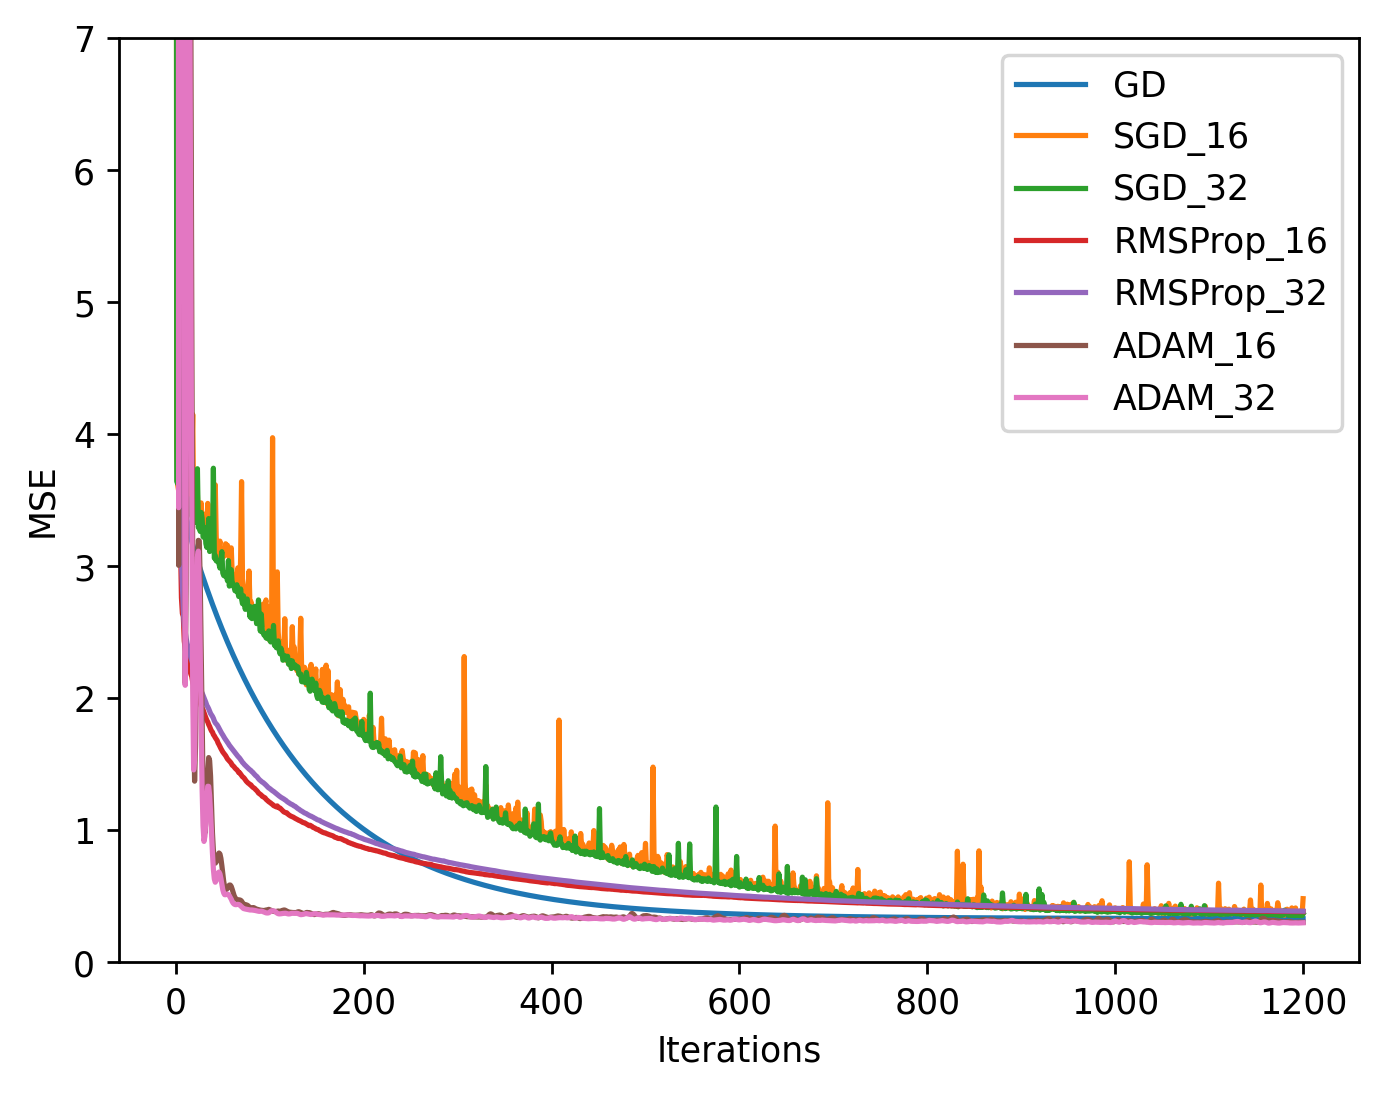
\includegraphics[width=\columnwidth]{pictures/wine_test_16_32}
	\caption{Test error for the wine dataset. Batch size one is left out for clarity.}
	\vspace{-3mm}
	\label{fig:wine_test_16_32}
\end{figure}


The progression of test errors over the training episodes, depicted in Figure ~\ref{fig:wine_test_16_32}, illustrates that Adam converges most rapidly. 
RMSProp exhibits initial quick convergence, but GD surpasses it as the training progresses. 
Furthermore, SGD exhibits less pronounced fluctuations with larger batch sizes. 
The evolution of the training error is nearly identical and is visualized in the appendix in Figure~\ref{fig:wine_train_16_32}.

Regarding the parameter tuning process, as outlined in table~\ref{tab:parameter_wine} in the appendix, it is recommended to utilize the best-performing versions of Adam and GD without regularization. 
Additionally, Adam's learning rate should be set at the upper limit of the permissible range. 
Only SGD reaches the minimum learning rate, while RMSProp tends to employ regularization more frequently.
The training time visualizes that GD needs the most time to optimize and smaller batch sizes mostly speed up the training progress.


\subsection{Bike Dataset}
The findings for the bike dataset differ from those of the wine dataset. This can be attributed to the larger range of the target variable in the bike dataset, resulting in higher mean squared error (MSE) values.

RMSProp emerged as the best-performing algorithm for the bike dataset, followed by Adam. In contrast, SGD ranked third, while GD lagged far behind in terms of performance. Notably, even after 100,000 training episodes, GD was unable to achieve the test error level of RMSProp.
A comprehensive summary of the results can be found in the appendix, in table~\ref{tab:bike_mses}.


\begin{figure}[tbp]
	\centering
	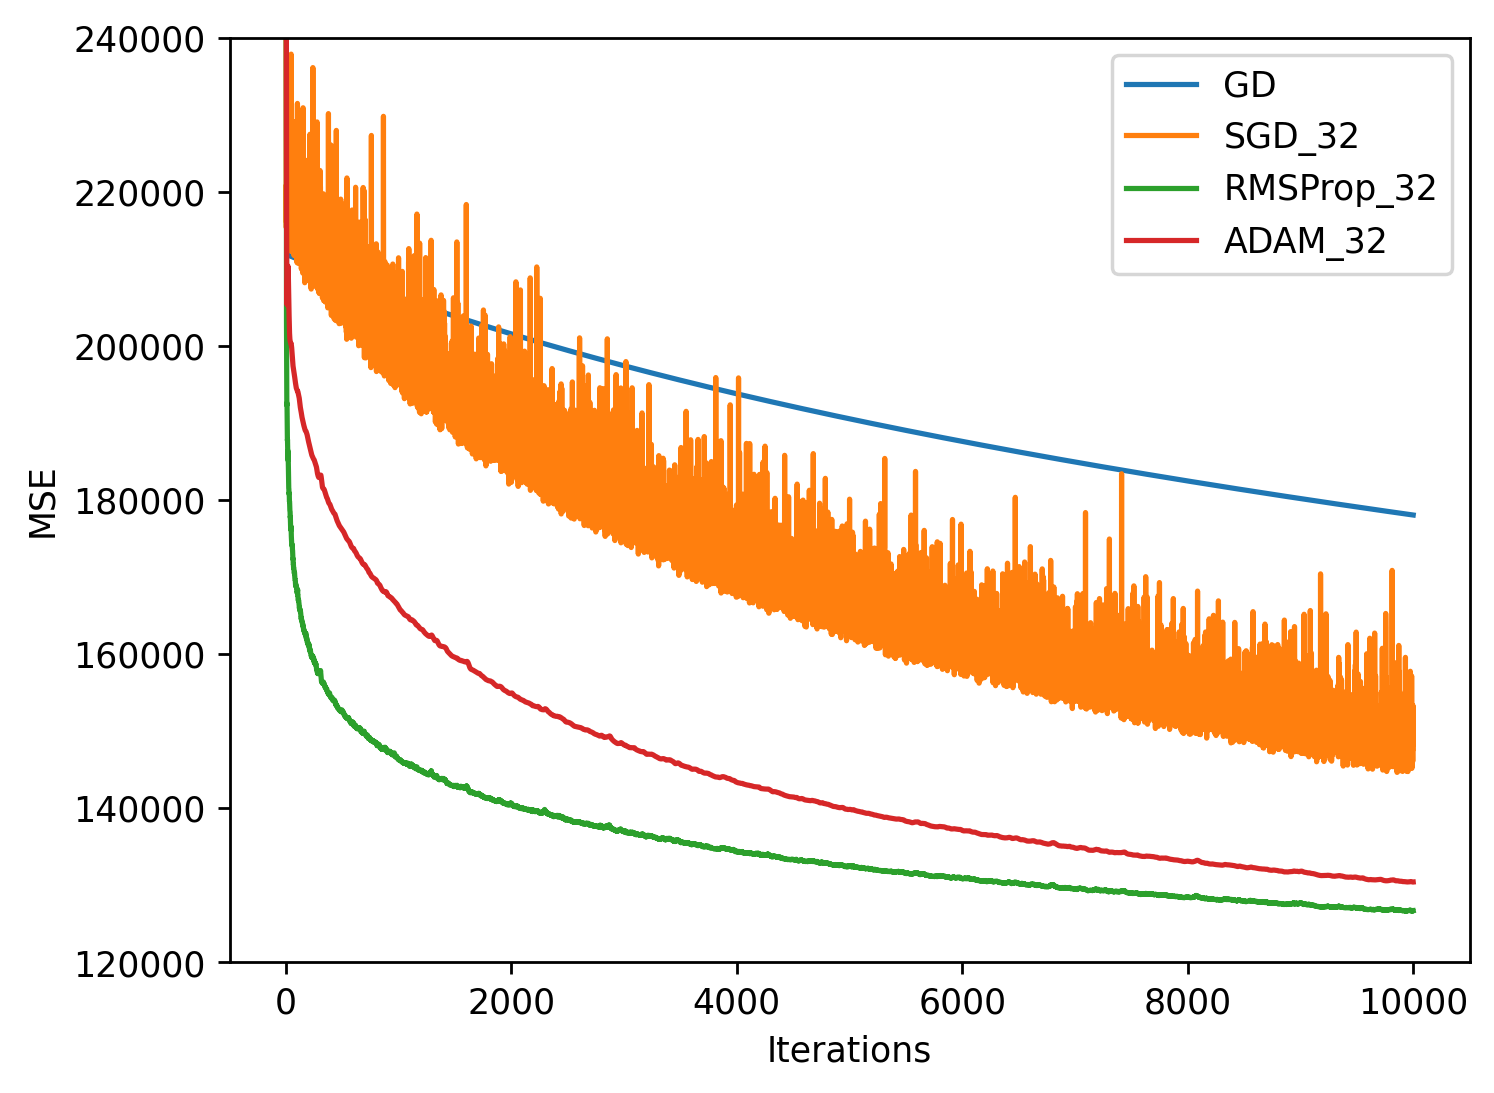
\includegraphics[width=\columnwidth]{pictures/bike_test_32}
	\caption{Test error for the bike dataset.}
	\vspace{-3mm}
	\label{fig:bike_test_32}
\end{figure}

The progression of the test error, depicted in figure~\ref{fig:bike_test_32}, illustrates that RMSProp exhibits rapid convergence, similar to Adam. 
On the other hand, GD shows a slower but more stable convergence, as observed in figure~\ref{fig:bike_test_GD_100k} in the appendix specifically for GD after 100,000 episodes. 
In contrast, SGD displays more pronounced fluctuations compared to the other algorithms.

The parameters obtained from the hyperparameter tuning process, presented in table~\ref{tab:parameter_bike} in the appendix, indicate that GD opts for the smallest possible learning rate without employing regularization. 
In contrast, both RMSProp and Adam choose the highest permissible learning rate while utilizing regularization.
This time GD is more than two times faster compared to all other variants.


\section{Conclusion}
The results confirm one of the greatest truths of computer science: It depends. 
Depending on the type of data and model, the different optimization algorithms perform differently concerning test errors.  
For the examples chosen in this paper with multiple linear regression and L1 regularisation, adaptive algorithms such as Adam and RMSProp seem to be the most suitable because they allow a faster convergence to the optimum. 
Of course, this depends on the type of model. 
If you choose a neural network as a model, the complexity is much higher. 
Here, adaptive algorithms can also overfit and be inferior to a fine-tuned SGD~\cite{wilson2018marginal}.

It also became clear that a stochastic approach can greatly accelerate learning, while the simple GD does not produce worse results but usually takes longer. 
The only exception to this is the result for the runtime for the bike dataset, but this could also be the fault of the scheduler.
On the other hand, GD converges quite steadily and is not subject to such fluctuations and, in contrast to all other methods, is deterministic.
The advantage of the adaptive methods is also evident in the comparison with SGD, where there are strong fluctuations between the episodes, and the adaptive methods are more stable.
As a note, it should be mentioned here that RMSProp without a learning rate decrease starts to oscillate strongly after it has converged and sometimes delivers very poor results. 
The same is true for Adam, but not as much as RMSProp. 
Therefore, in this project the adaptive methods were only used with a learning rate decrease.

The conducted experiments exhibit certain limitations. 
Firstly, only a narrow set of parameters was tuned, imposing severe constraints on the variability of the tuning process. 
Additionally, alternative regularization techniques were not explored, and it is possible that extending the duration of certain episodes could have yielded different outcomes. 
Moreover, the documented runtimes are influenced by the platform and scheduler, rendering them subject to variations. 
Consequently, this study offers only a restricted perspective and warrants the need for more extensive experiments to obtain deeper insights.

The obtained results align with the existing literature, indicating that adaptive algorithms are effective in quickly achieving desirable outcomes. 
However, as the models become more complex and multiple optima exist, adaptive algorithms tend to overfit.
Although this phenomenon was not observed in this study due to the simplicity of the models used, it highlights the importance of selecting the appropriate algorithm, considering the interplay between model complexity, data characteristics, and hyperparameter choices, to achieve optimal generalization performance.

Overall, this study contributes to the understanding of the bias-variance trade-off and the impact of optimization algorithms on generalization. 
It emphasizes the need to carefully select and configure algorithms based on the specific characteristics of the problem at hand.



\bibliographystyle{IEEEtran}
\bibliography{literature}


\section*{Appendix}



The code for the experiments can be found on github: \href{https://github.com/cclosheim/Opt4MLProject.git}{https://github.com/cclosheim/Opt4MLProject.git}.


\begin{table*}[htbp]
	\centering
	\begin{tabular}[c]{lllll}
		\hline
		Algorithm&last train error& min train error& last test error& min test error\\
		\hline
		
		GD& 0.3257& 0.3257& 0.3263 &0.3263\\
		SGD\_1& 14.0067& 0.4364& 13.8638& 0.4324\\
		SGD\_16& 0.4745& 0.3505 &0.4783& 0.3516\\
		SGD\_32& 0.3597& 0.3493& 0.3619& 0.3493\\
		RMSProp\_1& 0.5016 &0.5016& 0.4991& 0.4991\\
		RMSProp\_16& 0.3785& 0.3785& 0.3799& 0.3799\\
		RMSProp\_32& 0.3826& 0.3826& 0.3837& 0.3837\\
		ADAM\_1& 0.3837& 0.3271& 0.3871& 0.3284\\
		ADAM\_16& 0.2983& 0.296& 0.2996& 0.2963\\
		ADAM\_32 &0.2937& 0.2922& 0.2957& 0.2934\\
		\hline
	\end{tabular}
	\caption{Parameters chosen in the inner CV loops for the wine dataset.}
	\label{tab:wine_mses}
\end{table*}
\begin{figure}[htbp]
	\centering
	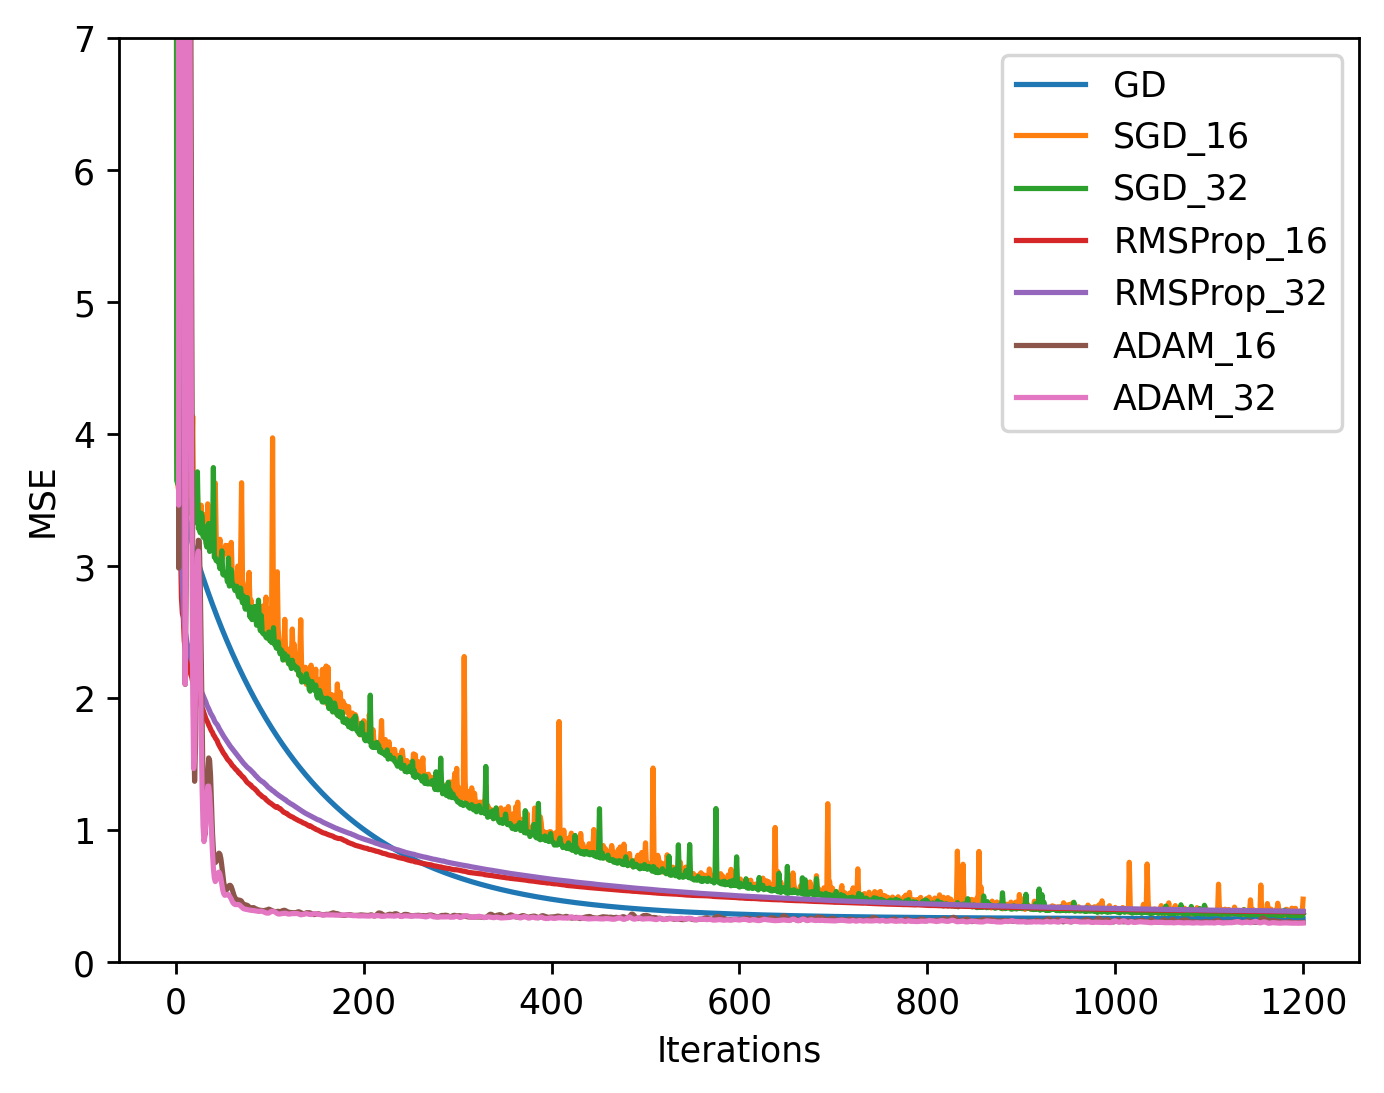
\includegraphics[width=\columnwidth]{pictures/wine_train_16_32}
	\caption{Train error for the wine dataset. Batch size one is left out for clarity.}
	\vspace{-3mm}
	\label{fig:wine_train_16_32}
\end{figure}


\begin{table*}[htbp]
	\centering
	\begin{tabular}[c]{llllllll}
		\hline
		Algorithm&Parameter&\#1&\#2&\#3&\#4&\#5&mean training time\\
		\hline
		
		\multirow{2}{*}{GD}&$\gamma$&0.0001&0.0001&0.0001&0.0001&0.0001&\multirow{2}{*}{30.0118}\\
							&$\lambda$&0&0&0&0&0&\\

		\multirow{2}{*}{SGD\_1}&$\gamma$&0.001&1e-06&0.01&1e-07&0.001&\multirow{2}{*}{5.4652}\\
								&$\lambda$&0.1&0&0&0&0&\\
		\multirow{2}{*}{SGD\_16}&$\gamma$&1e-07&0.0001&1e-07&0.001&1e-06&\multirow{2}{*}{17.7215}\\
								&$\lambda$&0.01&0&0&0&0&\\
		\multirow{2}{*}{SGD\_32}&$\gamma$&1e-05&0.01&0.001&0.001&1e-05&\multirow{2}{*}{21.2982}\\
								&$\lambda$&0&0&0&0&0.01&\\
			

		\multirow{2}{*}{RMSProp\_1}&$\gamma$&0.01&0.01&0.01&0.01&0.01&\multirow{2}{*}{13.1194}\\
									&$\lambda$&0.01&0&0.01&0&0.01&\\
		\multirow{2}{*}{RMSProp\_16}&$\gamma$&0.01&0.01&0.01&0.01&0.01&\multirow{2}{*}{19.6935}\\
									&$\lambda$&0.01&0&0.01&0.1&0.1&\\
		\multirow{2}{*}{RMSProp\_32}&$\gamma$&0.01&0.01&0.01&0.01&0.01&\multirow{2}{*}{26.1772}\\
									&$\lambda$&0.01&0&0.01&0&0.01&\\
		
		\multirow{2}{*}{Adam\_1}&$\gamma$&0.1&0.1&0.1&0.1&0.1&\multirow{2}{*}{16.3991}\\
								&$\lambda$&0&0&0.01&0&0.01&\\
		\multirow{2}{*}{Adam\_16}&$\gamma$&0.1&0.1&0.1&0.1&0.1&\multirow{2}{*}{21.8148}\\
								&$\lambda$&0&0&0&0&0&\\
		\multirow{2}{*}{Adam\_32}&$\gamma$&0.1&0.1&0.1&0.1&0.1&\multirow{2}{*}{19.2637}\\
								&$\lambda$&0&0&0&0&0&\\
		\hline
	\end{tabular}
	\caption{Parameters chosen in the inner CV loops for the wine dataset. The mean training time is the mean time over all training episodes for the best parameter sets.}
	\label{tab:parameter_wine}
\end{table*}



\begin{table*}[htbp]
	\centering
	\begin{tabular}[c]{lllll}
		\hline
		Algorithm&last train error& min train error& last test error& min test error\\
		\hline		
		GD &177952.4046 &177952.4046& 178023.0621& 178023.0621\\
		GD 100 episodes &127040.3122& 127040.3122 &127145.0298& 127145.0298\\
		SGD\_32& 147517.5138& 144393.933& 148258.3788& 144597.8354\\
		RMSProp\_32& 126403.1368 &126400.2521& 126634.0648& 126583.3529\\
		ADAM\_32& 130183.8598& 130183.8598& 130362.334 &130354.9358\\
		\hline
	\end{tabular}
	\caption{Parameters chosen in the inner CV loops for the wine dataset.}
	\label{tab:bike_mses}
\end{table*}




\begin{figure}[htbp]
	\centering
	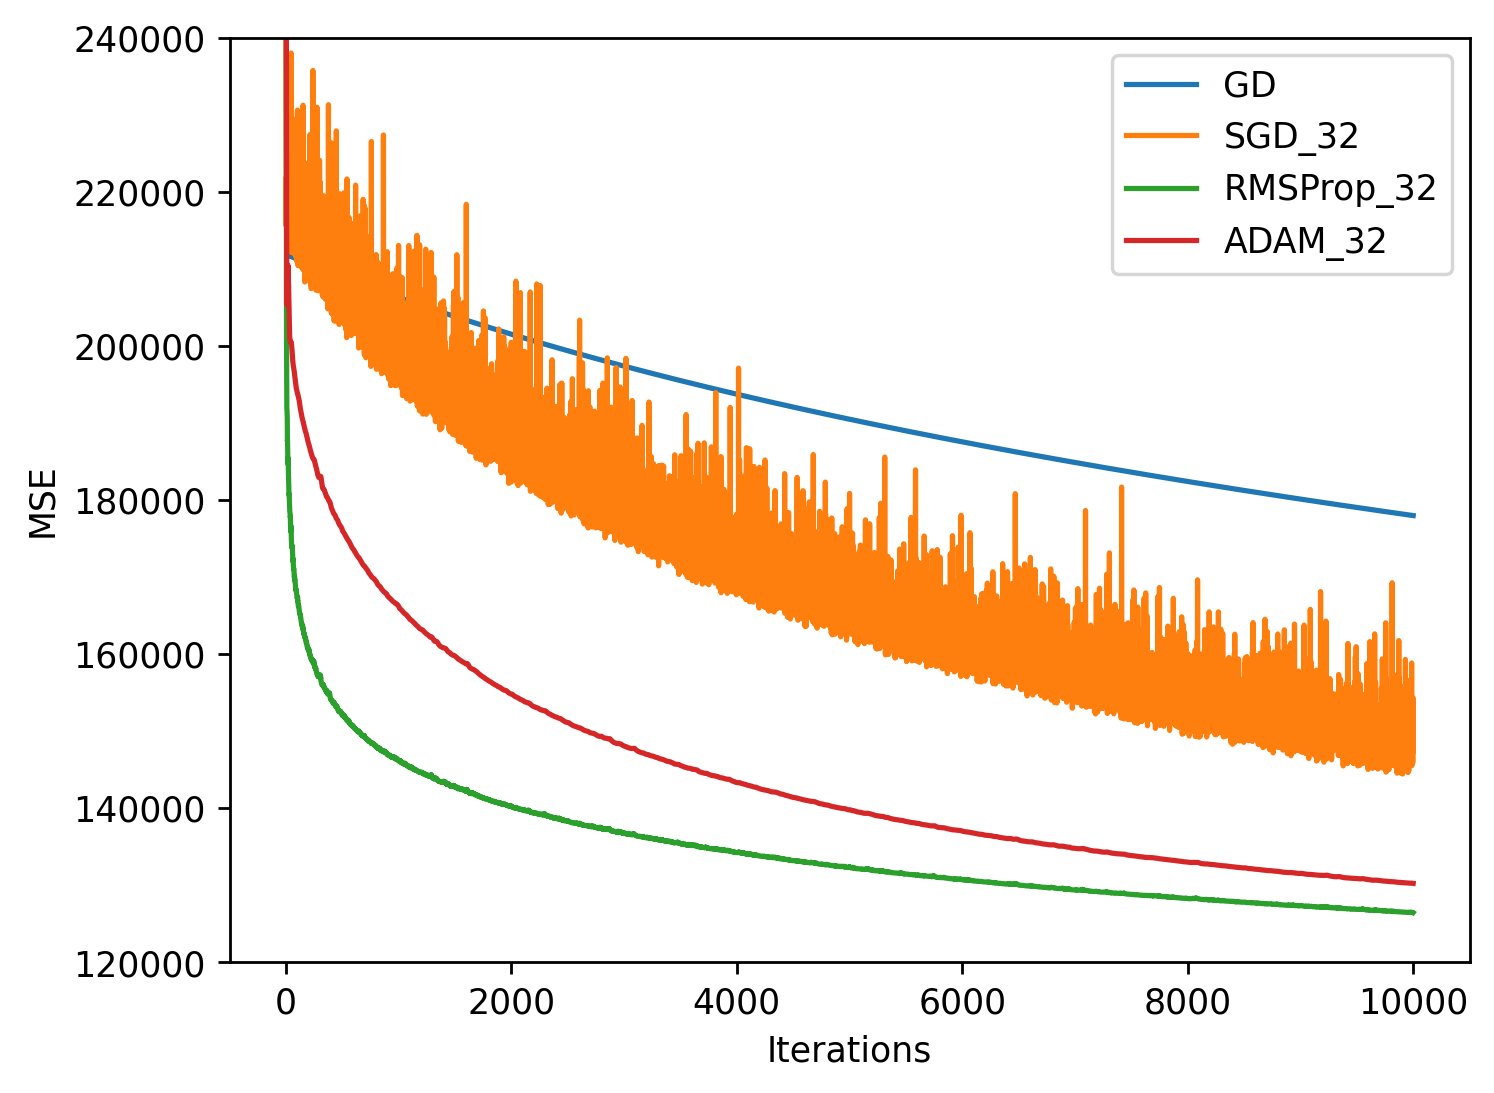
\includegraphics[width=\columnwidth]{pictures/bike_train_32}
	\caption{Train error for the bike dataset.}
	\vspace{-3mm}
	\label{fig:bike_train_32}
\end{figure}

\begin{figure}[htbp]
	\centering
	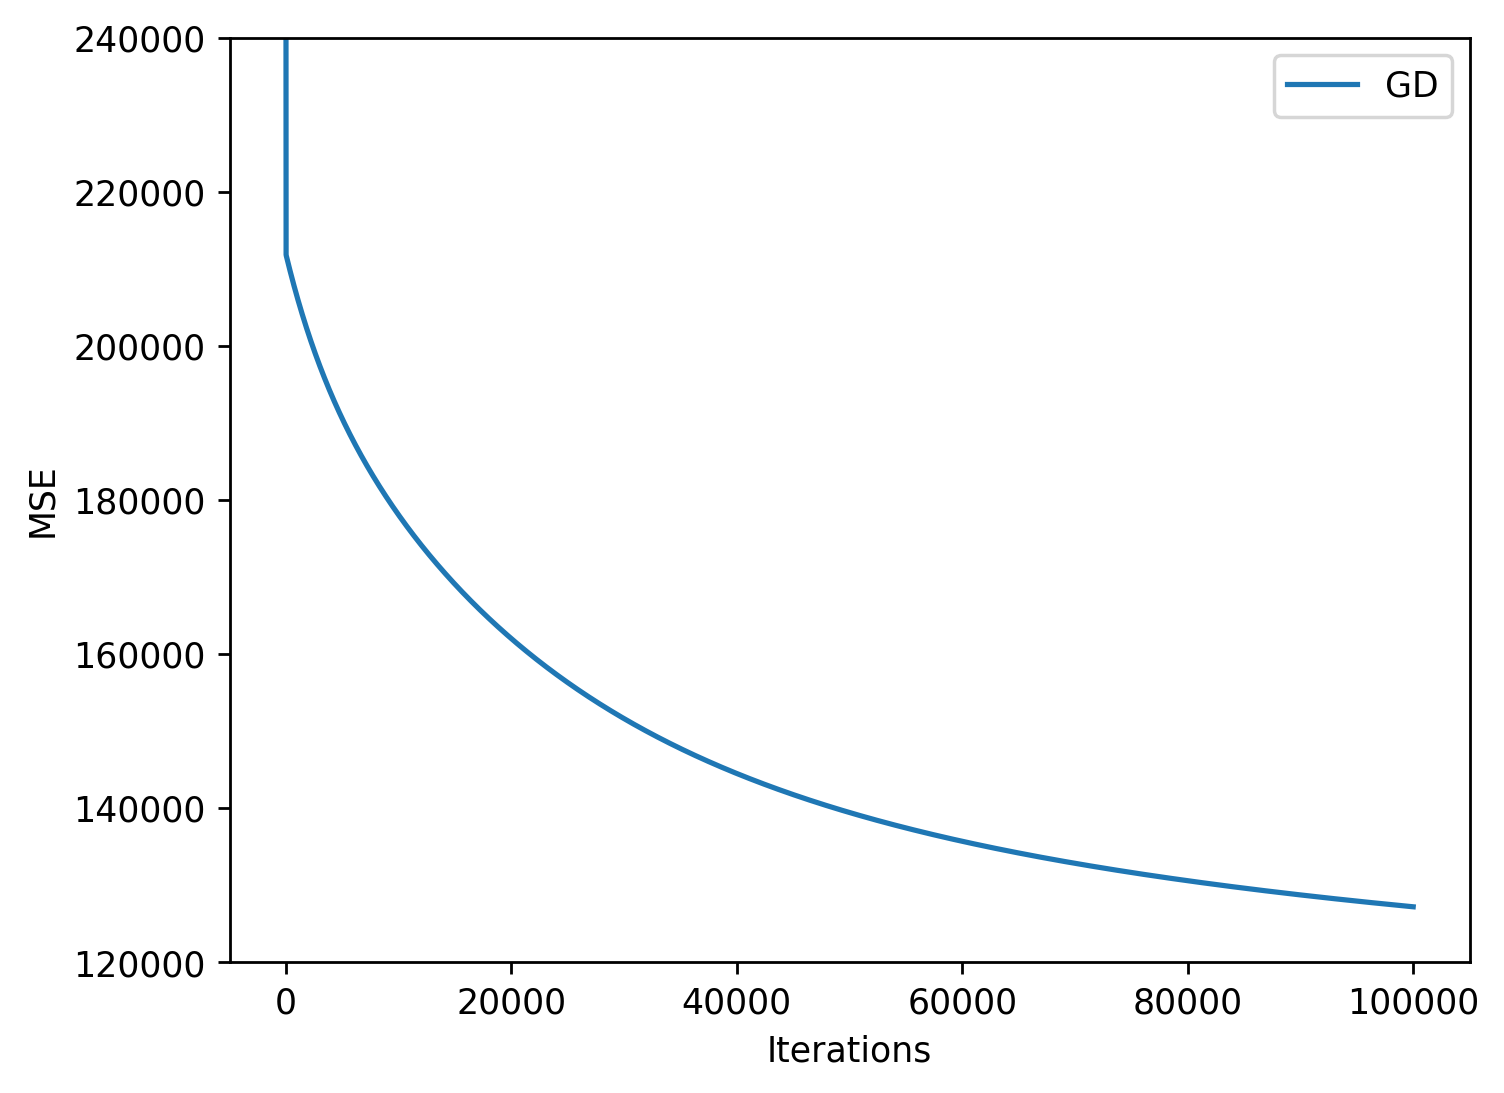
\includegraphics[width=\columnwidth]{pictures/bike_test_GD_100k}
	\caption{Test error for the bike dataset for GD on 100 thousands episodes.}
	\vspace{-3mm}
	\label{fig:bike_test_GD_100k}
\end{figure}

\begin{table*}[htbp]
	\centering
	\begin{tabular}[c]{llllllll}
		\hline
		Algorithm&Parameter&\#1&\#2&\#3&\#4&\#5&mean training time\\
		\hline
		\multirow{2}{*}{GD}&$\gamma$&1e-07&1e-07&1e-07&1e-07&1e-07&\multirow{2}{*}{15.679}\\
		&$\lambda$&0&0&0&0&0&\\
		
		\multirow{2}{*}{SGD\_32}&$\gamma$&0.01&0.1&0.001&0.001&1e-07&\multirow{2}{*}{40.1678}\\
		&$\lambda$&0.01&0&0.1&0.1&0.01&\\
		
		\multirow{2}{*}{RMSProp\_32}&$\gamma$&0.1&0.1&0.1&0.1&0.1&\multirow{2}{*}{45.9675}\\
		&$\lambda$&1&0&0.1&0&0.1&\\
		
		\multirow{2}{*}{Adam\_32}&$\gamma$&0.1&0.1&0.1&0.1&0.1&\multirow{2}{*}{46.5001}\\
		&$\lambda$&0&0.01&0&0&0.01&\\
		\hline
	\end{tabular}
	\caption{Parameters chosen in the inner CV loops for the bike dataset.}
	\label{tab:parameter_bike}
\end{table*}





\end{document}
